\chapter{Base de dados}

Como o approach foi decidido ser o Database First, criamos uma Base de Dados primeiro no SQL Server.

Para tal abrimos o SSMS e criamos uma Base de Dados com o mesmo nome do projecto, a qual abrimos uma Query onde listamos a estrutura e os dados iniciais.

\section{Notas}

A estrutura da base de dados foi a decidida anteriormente na analise de sistema, no então sofre umas alterações para que fosse possível a utilização do Entity Framework Core.

Estas alterações são o facto de todas as tabelas ter uma PK e qualquer FK tem de ter CASCADE (neste caso ON DELETE CASCADE).

\section{\textit{Query}}

\begin{lstlisting}[
    language=SQL,
    showspaces=false,
    basicstyle=\ttfamily,
    numbers=left,
    numberstyle=\tiny,
    commentstyle=\color{gray},
    breaklines=true
]

CREATE TABLE ingredients (i_id TINYINT PRIMARY KEY, name VARCHAR(32) NOT NULL);
CREATE TABLE tables (t_id TINYINT PRIMARY KEY, name VARCHAR(32) NOT NULL);
CREATE TABLE recipe (r_id TINYINT PRIMARY KEY, name VARCHAR(32) NOT NULL);
CREATE TABLE stock (
  i_id TINYINT PRIMARY KEY,
  quantity TINYINT NOT NULL,
  FOREIGN KEY (i_id) REFERENCES ingredients(i_id) ON DELETE CASCADE
);
CREATE TABLE rec_ing_list (
  ril_id TINYINT PRIMARY KEY,
  r_id TINYINT NOT NULL,
  i_id TINYINT NOT NULL,
  quantity TINYINT NOT NULL,
  FOREIGN KEY (r_id) REFERENCES recipe(r_id) ON DELETE CASCADE,
  FOREIGN KEY (i_id) REFERENCES ingredients(i_id) ON DELETE CASCADE
);
CREATE TABLE orders (
  o_id TINYINT PRIMARY KEY,
  date DATETIME NOT NULL,
  r_id TINYINT NOT NULL,
  FOREIGN KEY (r_id) REFERENCES recipe(r_id) ON DELETE CASCADE
);
CREATE TABLE tb_or_list (
  tol_id TINYINT PRIMARY KEY,
  o_id TINYINT NOT NULL,
  t_id TINYINT NOT NULL,
  quantity TINYINT NOT NULL,
  FOREIGN KEY (o_id) REFERENCES orders(o_id) ON DELETE CASCADE,
  FOREIGN KEY (t_id) REFERENCES tables(t_id) ON DELETE CASCADE
);
CREATE TABLE login_type (
  type_id TINYINT PRIMARY KEY,
  name VARCHAR(32) NOT NULL,
  chmod TINYINT NOT NULL
);
CREATE TABLE login (
  l_id TINYINT PRIMARY KEY,
  username VARCHAR(32) NOT NULL,
  passhash VARCHAR(32) NOT NULL,
  type_id TINYINT NOT NULL,
  FOREIGN KEY (type_id) REFERENCES login_type(type_id) ON DELETE CASCADE
);
CREATE TABLE reservation (
  res_id TINYINT PRIMARY KEY,
  t_id TINYINT NOT NULL,
  date DATETIME NOT NULL,
  l_id TINYINT NOT NULL,
  FOREIGN KEY (t_id) REFERENCES tables(t_id) ON DELETE CASCADE,
  FOREIGN KEY (l_id) REFERENCES login(l_id) ON DELETE CASCADE
);
INSERT INTO recipe (r_id, name)
VALUES (1, 'Cake'),
  (2, 'Cookie'),
  (3, 'Pancake'),
  (4, 'Pie');
INSERT INTO ingredients (i_id, name)
VALUES (1, 'Flour'),
  (2, 'Sugar'),
  (3, 'Eggs'),
  (4, 'Milk'),
  (5, 'Butter'),
  (6, 'Baking Powder'),
  (7, 'Salt'),
  (8, 'Vanilla'),
  (9, 'Cake Mix'),
  (10, 'Cookie Mix'),
  (11, 'Pancake Mix'),
  (12, 'Pie Mix');
INSERT INTO rec_ing_list (ril_id, r_id, i_id, quantity)
VALUES (1, 1, 1, 1),
  (2, 1, 2, 1),
  (3, 1, 3, 1),
  (4, 2, 4, 1),
  (5, 2, 5, 1),
  (6, 2, 6, 1),
  (7, 3, 7, 1),
  (8, 3, 8, 1),
  (9, 3, 9, 1),
  (10, 4, 10, 1),
  (11, 4, 11, 1),
  (12, 4, 12, 1);
INSERT INTO stock (i_id, quantity)
VALUES (1, 74),
  (2, 115),
  (3, 46),
  (4, 40),
  (5, 63),
  (6, 124),
  (7, 117),
  (8, 93),
  (9, 85),
  (10, 135),
  (11, 120),
  (12, 191);
INSERT INTO login_type (type_id, name, chmod)
VALUES (1, 'Admin', 1),
  (2, 'Manager', 2),
  (3, 'Employee', 3),
  (4, 'Customer', 4);
INSERT INTO login (l_id, username, passhash, type_id)
VALUES (1, 'admin', 'admin', 1),
  (2, 'manager', 'manager', 2),
  (3, 'employee', 'employee', 3),
  (4, 'customer', 'customer', 4);
INSERT INTO tables (t_id, name)
VALUES (1, 'Table 1'),
  (2, 'Table 2'),
  (3, 'Table 3'),
  (4, 'Table 4'),
  (5, 'Table 5'),
  (6, 'Table 6'),
  (7, 'Table 7'),
  (8, 'Table 8'),
  (9, 'Table 9'),
  (10, 'Table 10');
INSERT INTO reservation (res_id, t_id, date, l_id)
VALUES (1, 6, '2022-01-17 17:00:00', 1),
  (2, 7, '2022-01-17 18:30:0', 1),
  (3, 8, '2022-01-17 19:30:00', 1),
  (4, 9, '2022-01-18 13:00:00', 1),
  (5, 10, '2022-01-19 12:30:00', 1);
INSERT INTO orders (o_id, date, r_id)
VALUES (1, '2022-01-17 17:00:00', 1),
  (2, '2022-01-17 18:30:0', 1),
  (3, '2022-01-17 19:30:00', 1),
  (4, '2022-01-18 13:00:00', 1),
  (5, '2022-01-19 12:30:00', 1);
INSERT INTO tb_or_list (tol_id, o_id, t_id, quantity)
VALUES (1, 1, 6, 1),
  (2, 2, 7, 1),
  (3, 3, 8, 1),
  (4, 4, 9, 1),
  (5, 5, 10, 1);

\end{lstlisting}

\newpage
\section{Conteúdo Gerado}

A \textit{Query} no final da execução gerou a base de dados com a seguinte estrutura:

\begin{figure}[!hbt]
    \centering
    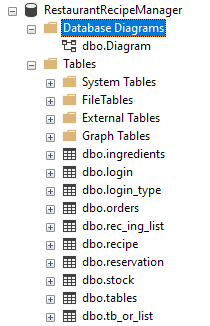
\includegraphics[width=6cm]{Resources/Database/DB (2).png}
    \caption{Tabelas Geradas}
    
\end{figure}

A qual melhor demonstrada via este Diagrama:

\begin{figure}[!hbt]
    \centering
    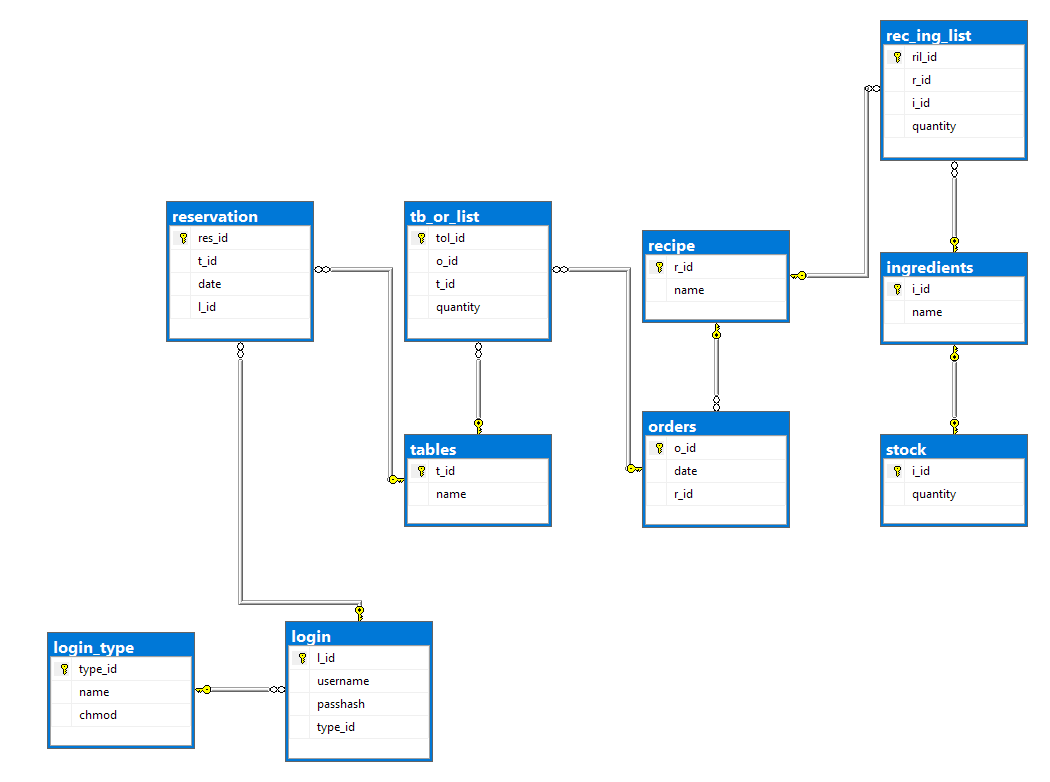
\includegraphics[width=14cm]{Resources/Database/DB (1).png}
    \caption{Diagrama da base de dados}
    
\end{figure}